\documentclass[11pt]{article}
\usepackage{graphicx}
\usepackage{hyperref}
\usepackage{amsmath}
\usepackage{amsthm}
\usepackage{amssymb}
\usepackage[all=normal,floats,leading,paragraphs,charwidths,tracking,wordspacing]{savetrees}
\usepackage{float}
\usepackage[version = 4]{mhchem}
\usepackage{multirow}
\usepackage{commath}
\usepackage{booktabs}
\usepackage{subcaption}
\renewcommand{\arraystretch}{1.2}
\usepackage{siunitx}
\sisetup{detect-all}
\usepackage{listings}
\usepackage{color} %red, green, blue, yellow, cyan, magenta, black, white
\definecolor{mygreen}{RGB}{28,172,0} % color values Red, Green, Blue
\definecolor{mylilas}{RGB}{170,55,241}
\usepackage[a4paper,margin=15mm]{geometry}
\numberwithin{equation}{section}
\setlength{\parskip}{\baselineskip}
\setlength{\parindent}{0pt}
\hypersetup{
    colorlinks=true,
    linkcolor=black,
    filecolor=black,      
    urlcolor=black,
    citecolor=black
}
\urlstyle{same}
\lstset{language=Matlab,%
    %basicstyle=\color{red},
    breaklines=true,%
    morekeywords={matlab2tikz},
    keywordstyle=\color{blue},%
    morekeywords=[2]{1}, keywordstyle=[2]{\color{black}},
    identifierstyle=\color{black},%
    stringstyle=\color{mylilas},
    commentstyle=\color{mygreen},%
    showstringspaces=false,%without this there will be a symbol in the places where there is a space
    numbers=left,%
    numberstyle={\tiny \color{black}},% size of the numbers
    numbersep=9pt, % this defines how far the numbers are from the text
    emph=[1]{for,end,break},emphstyle=[1]\color{red}, %some words to emphasise
    %emph=[2]{word1,word2}, emphstyle=[2]{style},    
}
\begin{document}
\title{\textbf{UCL Mechanical Engineering 2021/2022}\\MECH0024 Coursework}
\author{RFLH9}
\date{\today}
\maketitle
\tableofcontents
\listoffigures
\newpage
\part{SpaceX rocket engine essay}
SpaceX has been developing rocket engines for nearly two decades. The two primary engine families being developed today are the Merlin series and the Raptor series. The Draco and SuperDraco series of engines have also been developed by SpaceX, however their role as Reaction Control System (RCS) thrusters and Launch Abort System engines respectively leave them to be not considered in this essay. SpaceX has developed these rocket engines to power a variety of booster rockets, including the Falcon 9, Falcon Heavy and Starship. The roles of these rockets include delivering crew and cargo to space, as well as interplanetary travel. SpaceX places a strong emphasis on reusability and a reduction of `cost to launch'. Hence, the engines powering these flights must be efficient, powerful and reliable to facilitate multiple missions.

The Merlin series powers the Falcon 9 and Falcon Heavy rocket boosters. These are two-stage rockets, designed to place cargo and crew into earth orbit. The first stage is powered by nine Merlin `sea level' engines and the second stage is powered by one Merlin `vacuum' engine. There have been a variety of developments over the past years and the current generation of Merlin engines is the Merlin 1D. The Merlin 1D uses an open-cycle gas-generator cycle with Rocket Propellant 1 (RP-1) and liquid oxygen (LOX) as propellants.

The fuel choice for the Merlin engine is due to a large variety of factors. The Merlin engine uses liquid propellants for combustion. RP-1 is a refined kerosene with low amounts of impurities and has been a widely used choice for the past 70 years. It is a liquid at room temperature, safe to handle, cheap and available in large quantities. This makes it ideal for rockets which need to fly frequently (as the Falcon rockets do). However, RP-1 is not the most efficient fuel as liquid Hydrogen (LH2) has a far greater specific impulse (\SI{289}{\second} vs \SI{381}{\second}) but RP-1 has greater density (\SI{0.071}{\gram\per\mol} vs \SI{0.82}{\gram\per\mol}) \cite{b1}. Another disadvantage of RP-1 is that it is a hydrocarbon, resulting in carbon deposits when burnt at the improper fuel-oxidiser ratio. This can lead to a build up of carbon deposits in the engine, decreasing the lifetime of the engine. Some alternatives to RP-1 include LH2 and liquid Methane. These two fuels are sometimes referred to as cryogenic fuels as their boiling points are far below room temperature and require more complex pressurised tanks and plumbing within the engine, presenting a different set of engineering challenges. After passing through the turbopumps, the propellants are driven through a pintle type injector and combusted in the main chamber.

\begin{figure}[H]
    \centering
    \begin{minipage}{.5\textwidth}
        \centering
        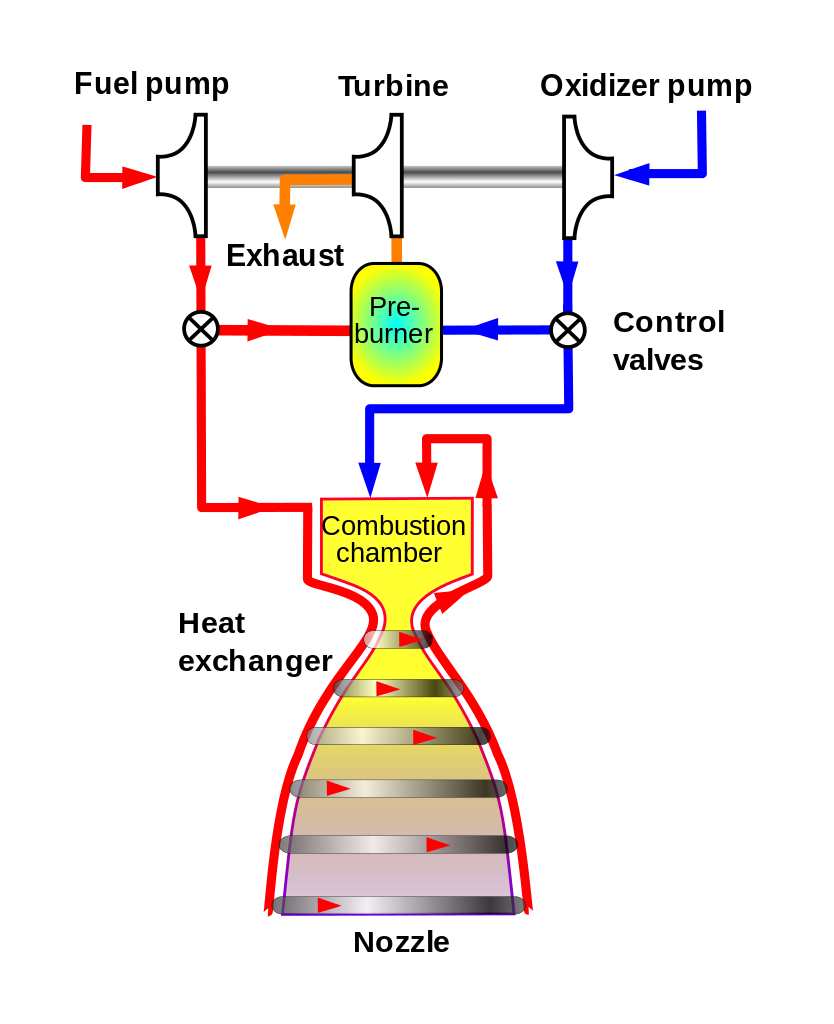
\includegraphics[height = 30ex]{./img/openCycle.png}
        \captionof{figure}{Open-cycle gas-generator cycle \cite{b2}.}
        \label{gasGeneratorCycle}
    \end{minipage}%
    \begin{minipage}{.5\textwidth}
        \centering
        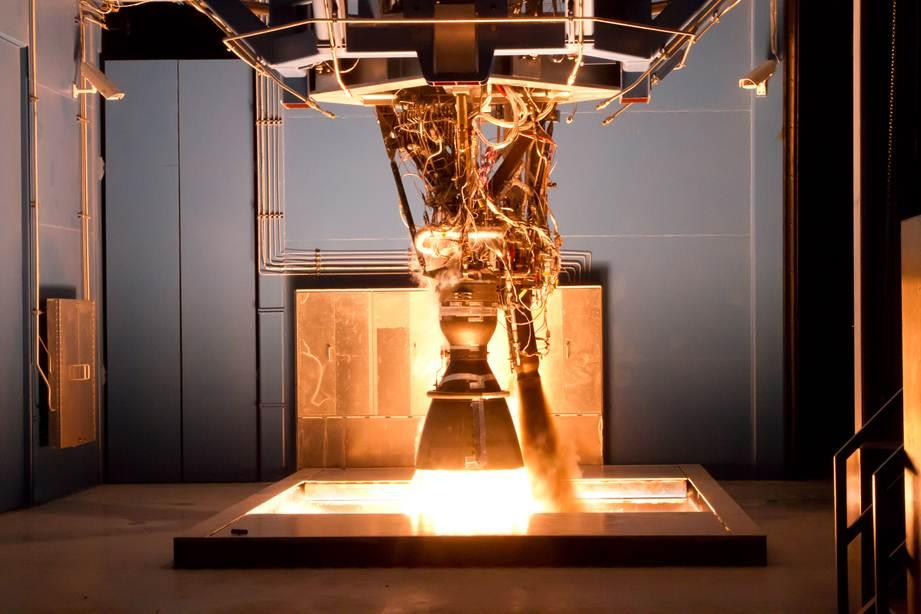
\includegraphics[height = 30ex]{./img/merlinTest.jpg}
        \captionof{figure}{Merlin engine test fire. Note the sooty exhaust on the right side from the preburner and turbine \cite{b3}.}
        \label{merlinTest}
    \end{minipage}
\end{figure}

To dissect the combustion cycle of the Merlin engine, let us take a look at how the engine is designed. In Figure \ref{gasGeneratorCycle}, we see that RP-1 and LOX is fed through turbopumps powered by a turbine on a single shaft. The turbine is driven by hot gas from a `preburner'. Some of the fuel and oxidiser is tapped off before it reaches the main combustion chamber for preburner combustion. After passing through the turbine, the gas is exhausted overboard. We see this as the sooty exhaust in Figure \ref{merlinTest}. The presence of soot in the preburner exhaust is evidence of a fuel rich fuel-oxidiser ratio. As the combustion products from the preburner are not used in the main combustion chamber, we have a definitive loss in efficiency as we are not utilising all of our fuel for main engine thrust. We refer to this as an `open-cycle'. Another issue to contend with is shaft leak. This is where the fuel rich gas from the preburner can seep through the shaft interpropellant seal towards the oxidiser turbopump. This may cause combustion before the propellants reach the main combustion chamber, reducing efficiency.

\begin{figure}[H]
    \centering
    \begin{minipage}{.5\textwidth}
        \centering
        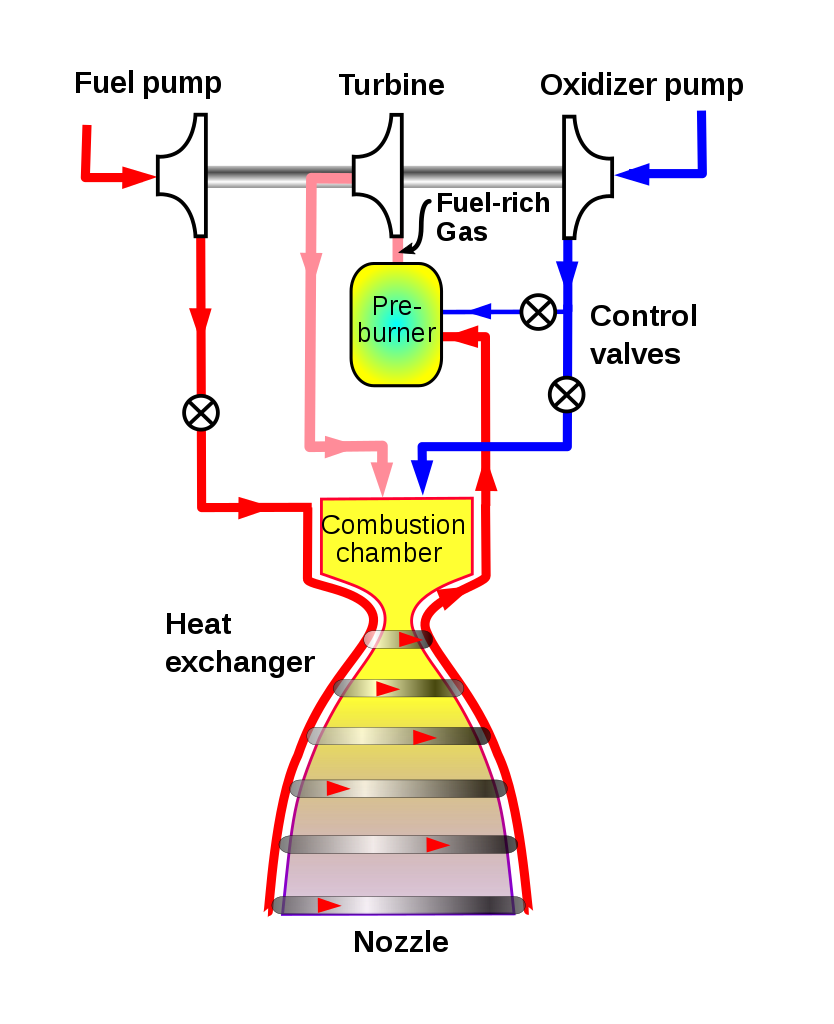
\includegraphics[height = 30ex]{./img/closedCycle.png}
        \captionof{figure}{Closed-cycle staged combustion cycle \cite{b4}.}
        \label{closedCycle}
    \end{minipage}%
    \begin{minipage}{.5\textwidth}
        \centering
        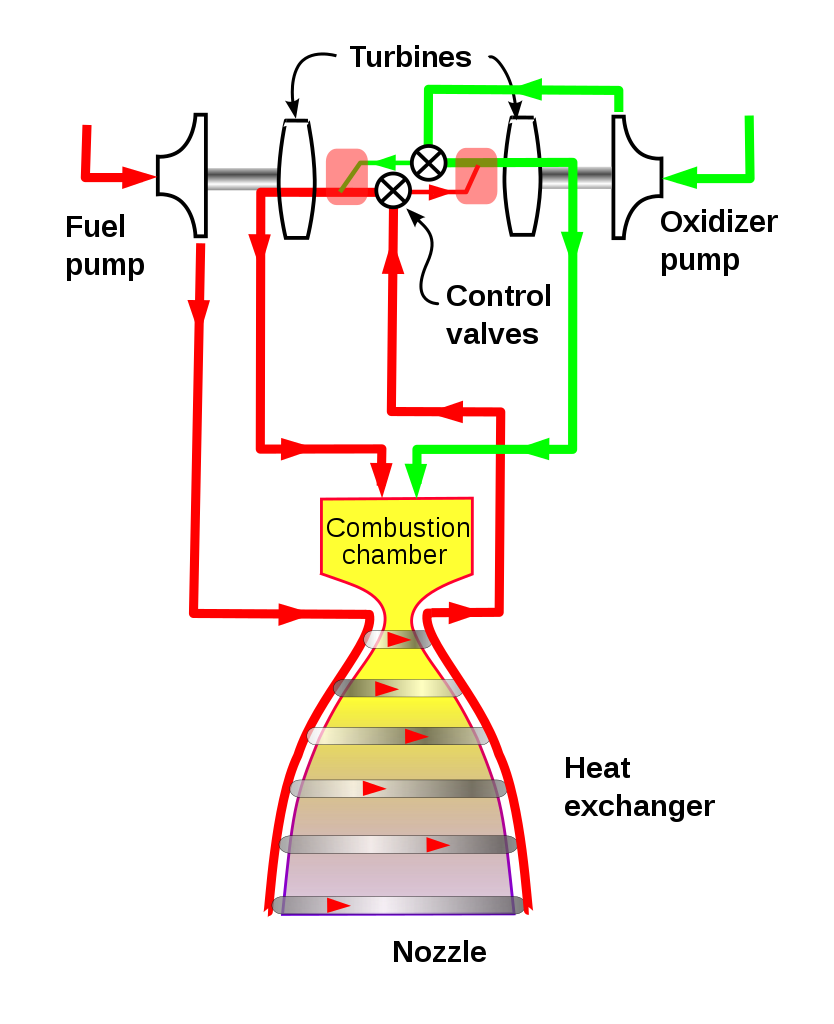
\includegraphics[height = 30ex]{./img/fullFlowCycle.png}
        \captionof{figure}{Full-flow staged combustion cycle \cite{b5}.}
        \label{fullFlow}
    \end{minipage}
\end{figure}

To improve the efficiency of this cycle, we can feed the exhaust from the turbine into our main combustion chamber `closing our cycle'. This is also called a staged combustion cycle and Figure \ref{closedCycle} shows a general closed-cycle staged combustion cycle. This presents an engineering problem as the main combustion chamber will exert pressure back through to the turbine and pre-burner. To solve this problem, the preburner needs to generate more energy and higher pressures to better match the pressure within the main combustion chamber. The turbine will need to withstand higher temperatures and larger stresses, requiring advanced metallurgy. The Merlin engine reduces the stress on its turbine by running fuel rich as this reduces the combustion temperature. As our fuel is hydrocarbon based, we run the risk of `coking' where carbon deposits clog the plumbing within the engine. We can run our preburner oxidiser rich (e.g. NPO Energomash RD-180 engine \cite{b6}) but this results in an exhaust which is chemically corrosive, due to the presence of high temperature oxygen. Higher pressures and temperatures will also exacerbate our shaft leak problem, requiring tighter engineering tolerances. Closed-cycle staged combustion cycle engines are more efficient but have more complex designs, leading to added weight and an increased cost to manufacture and maintain. A balance must be struck to ensure that these engines are viable.

The SpaceX Raptor engine utilises a full-flow staged combustion cycle (Figure \ref{fullFlow}) with liquid Methane and liquid Oxygen as propellants. Liquid Methane has a higher specific impulse than RP-1 but still not as high as LH2 \cite{b1}. Similar to RP-1, liquid Methane is more dense and can be cryonically stored in the tanks to increase volume of fuel onboard. As Methane is a smaller hydrocarbon than kerosene, it burns much cleaner, reducing the effect of the coking problem with RP-1. It is also abundant and can be easily made on other planets.

In the full-flow design, we see two separate turbines powering each turbopump. This separates our fuel-rich and oxidiser-rich gases, eliminating the need for interpropellant seals along our shafts. This design requires less energy per turbine as it only has to power one turbompump, leading to cooler preburner temperatures. This improves turbine life and reliability. By the time the propellants reach the combustion chamber, the propellants are gases, due to heating from the preburners. Gaseous propellants improve efficiency as you no longer have to force liquid propellants through an injector (which takes energy away from the propellants); the gases can mix very rapidly and efficiently in the main chamber. We also see higher mass flow rates as all the fuel and oxidiser is used in the main combustion chamber. This allows for a reduction in the pressures required, leading to even lower temperatures and lower stresses on the engine, improving reusability. The full-flow cycle is even more complex than the closed-cycle, as each preburner is reliant on the other. This requires precise engine control and a fast start-up sequence of both preburners to prevent an imbalance in fuel/oxidiser ratio.

A novel design of the SpaceX engines is the use of subcooled propellants. When the propellants are closer to their freezing points, their densities are higher. When passing the propellants through the turbopumps, we may see cavitation at the tips of the impeller blades if the propellant is close to its boiling point (due to high pressures). By subcooling the propellant, we can lower our RPM and still deliver the same mass flow rate (due to higher propellant density). This reduces the risk of cavitation as a lower tip speed will lead to a lower pressure differential, decreasing the risk of cavitation. The Raptor engine heavily incorporates 3D printed components. An estimated 40\% of the components on the Raptor engine are 3D printed \cite{b7}. Both Merlin and Raptor engines use components which are heavily vertically integrated within SpaceX. Compared to rocket engines built by other manufacturers, where components are built by numerous contractors, SpaceX engine components are almost all designed and built in-house, reducing cost and allowing for a high level of customisability.

All of these developments allow for SpaceX engines to be reliable and powerful, having been used and reused many times on Falcon and Starship rocket flights.
\part{Sea Level and Vacuum Merlin 1D rocket engines analysis}
\section{}
\subsection{Estimation of ideal OF ratio \& comparison with typical value}
Using Kerosene and Oxygen as our propellants, our chemical balance is:
\begin{equation}
    \ce{C12H4 + 36O2 -> 12H2O + 12CO2}
\end{equation}
Therefore, oxidiser fuel ratio by mass is:
\begin{gather}
    \textrm{OF}_{stoi} = \dfrac{18 (\SI{32}{\gram\per\mol})}{12(\SI{12}{\gram\per\mol}) + 24(\SI{1}{\gram\per\mol})} = \dfrac{576}{168} = 3.429
\end{gather}
A typical value for RP-1 LOX rocket engines is given as $\textrm{OF}_{typ} = 2.3$. This tells us that these engines run fuel rich. Richard Nakka derives \ref{exitVel} \cite{b8}:
\begin{gather}
    v_e = \sqrt{2 T_0 \left(\frac{R'}{M}\right)\left(\frac{k}{k-1}\right)\left[1 - \left(\frac{P_e}{P_0}\right)^{\frac{k-1}{k}}\right]} \label{exitVel}
\end{gather}
where:
\begin{itemize}
    \item $v_e$ is the exit velocity at the nozzle of the engine.
    \item $T_0$ is the combustion temperature of propellant.
    \item $R' = \SI{8314}{\joule\per\kilo\mol\per\kelvin}$ is the universal gas constant.
    \item $M$ is the effective molecular weight of exhaust products.
    \item $k$ effective ratio of specific heats of exhaust products.
    \item $P_e$ is nozzle exit pressure.
    \item $P_0$ is chamber pressure.
\end{itemize}
Here we can see that if we decrease the molecular weight of our exhaust, we increase our nozzle velocity. This makes it desirable to have lighter exhaust products. In the case of RP-1 LOX combustion, it would be preferable to have \ce{CO} mixed into our exhaust alongside \ce{H20} and \ce{CO2}, as this would reduce the molecular weight of the exhaust. Running fuel rich ensures that all of the oxygen is used for combustion, increasing overall efficiency. We must be careful to fine tune our OF ratio, as running too fuel rich may leave unburnt kerosene in the exhaust (which is quite heavy) and even the partial combustion to \ce{CO} is less energetic.

We may also want to run fuel rich to lower our combustion temperature. If our combustion temperature is too hot, we risk damaging components in the engine. It also ensures that we do not have unburned, hot oxidiser (which is corrosive towards metals) damaging engine components.
\subsection{Estimation of isentropic index $\gamma$}
test
\subsection{Estimation of molecular weight of combustion products $M_g$}
test
\subsection{Estimation of heat capacity $c_p$}
test
\subsection{Estimation of the adiabatic flame temperature of the combustion product in the combustion chamber}
test
\section{Determination of mass flux through both rocket engines}
test
\section{Estimation of exit velocity of jet exhaust in both cases}
test
\section{Estimation of exit pressure of the exhaust in both cases}
test
\section{}
\subsection{Estimation of  rocket thrust for the Sea Level Merlin 1D during the initial take-off and the Vacuum Merlin 1D operating in space}
test
\subsection{Estimation of the specific impulse in both cases}
test
\subsection{Discussion of differences between estimations and reported values}
test
\section{Sketch of exit flow/shock expansion fan characteristics}
\subsection{At sea level}
test
\subsection{At an altitude of \SI{5.5}{\kilo\meter}}
test
\section{Description of other technologies (and their working principles), which accommodate the change in back-pressure on thrust performance}
test
\begin{thebibliography}{00}
    \bibitem{b1} Robert A. Braeunig, (2008) `Rocket Propellants' \url{http://www.braeunig.us/space/propel.htm} Accessed: 14/12/2021
    \bibitem{b2} Duk, (2016) `Gas Generator Rocket Cycle' \url{https://commons.wikimedia.org/wiki/File:Gas_generator_rocket_cycle.svg}; see also \url{https://commons.wikimedia.org/wiki/User:Duk}, CC BY-SA 3.0, Accessed 15/12/2021
    \bibitem{b3} SpaceX. (2012) `Merlin 1D Test Fire' \url{http://www.spacex.com/media-gallery/detail/1661/172}; see also \url{http://www.spacex.com/news/2013/03/26/merlin-engines}, CC0, \url{https://commons.wikimedia.org/w/index.php?curid=46487822} Accessed: 15/12/2021
    \bibitem{b6} Mark Wade, (2019) `RD-180' \url{http://www.astronautix.com/r/rd-180.html} Accessed: 15/12/2021
    \bibitem{b4} Duk, (2017) `Staged Combustion Cycle' \url{https://commons.wikimedia.org/wiki/File:Staged_combustion_rocket_cycle.svg#filelinks}; see also \url{https://commons.wikimedia.org/wiki/User:Duk}, CC BY-SA 3.0, Accessed 15/12/2021
    \bibitem{b5} Duk, (2021) `Staged Combustion Cycle' \url{https://commons.wikimedia.org/wiki/File:Full_flow_staged_rocket_cycle.svg}; see also \url{https://commons.wikimedia.org/wiki/User:Duk}, CC BY-SA 3.0, Accessed 15/12/2021
    \bibitem{b7} Alejandro G. Belluscio, (2016) `The evolution of the SpaceX Raptor engine' \url{https://www.nasaspaceflight.com/2016/10/its-propulsion-evolution-raptor-engine/} Accessed: 15/12/2021
    \bibitem{b8} Richard Nakka, (2015) `Solid Rocket Motor Theory -- Nozzle Theory' \url{http://www.nakka-rocketry.net/th_nozz.html} Accessed: 15/12/2021
\end{thebibliography}
\end{document}